\section{Introduction}{
\par\noindent Nowadays, many model aircraft need  to be routinely tested and evaluated in the model plane airports(e.g., HKMEC air field in Figure \ref{HKMEC}. Model plane airports, similar to airports designed for real airplanes, also seek to minimize the waiting time for each individual airplane by carefully considering the current time, availability of the runway, and position of each airplane. The delivery of the airplane to a specific position is always an important task for the model plane airport, but it often consumes a lot of time and human resources. Specifically, the model planes need to be placed on the runway before taking off and manually dragged from the runway after landing. 

\par\noindent Due to the fact that the process of dragging the model airplane to a predefined location is highly repetitive and time-consuming, it is reasonable to then propose a tractor similar to the tractor in real airports as shown in Figure \ref{real_tractor}. The tractor in this case should be generally replace the task as performed by human in the past. Thus, in order to accomplish these tasks, there are several goals or requirements of this project: 1. The airplane should be almost automatic, and people only need to predefine the starting point and ending point beforehand. 2. The tractors are able to handle diversified airplanes with different parameters like height. 3. The airplane should be hard enough in material so as to avoid short-time maintenance and even replacement. Under these initiatives, we made our own version of autonomous towing tractor for model airfields. Our car has the following functions: 1. Detect and locate the target airplane in the airfield. 2. Grab the handle of the airplane and release it in the end through robot arm and mechanical claw. 3. Track the light spot as installed right before the landing gear. 4. Send real-time data, such as humidity and pressure, to the airplane.



\begin{figure}[h]
    \begin{minipage}{0.43\linewidth}
        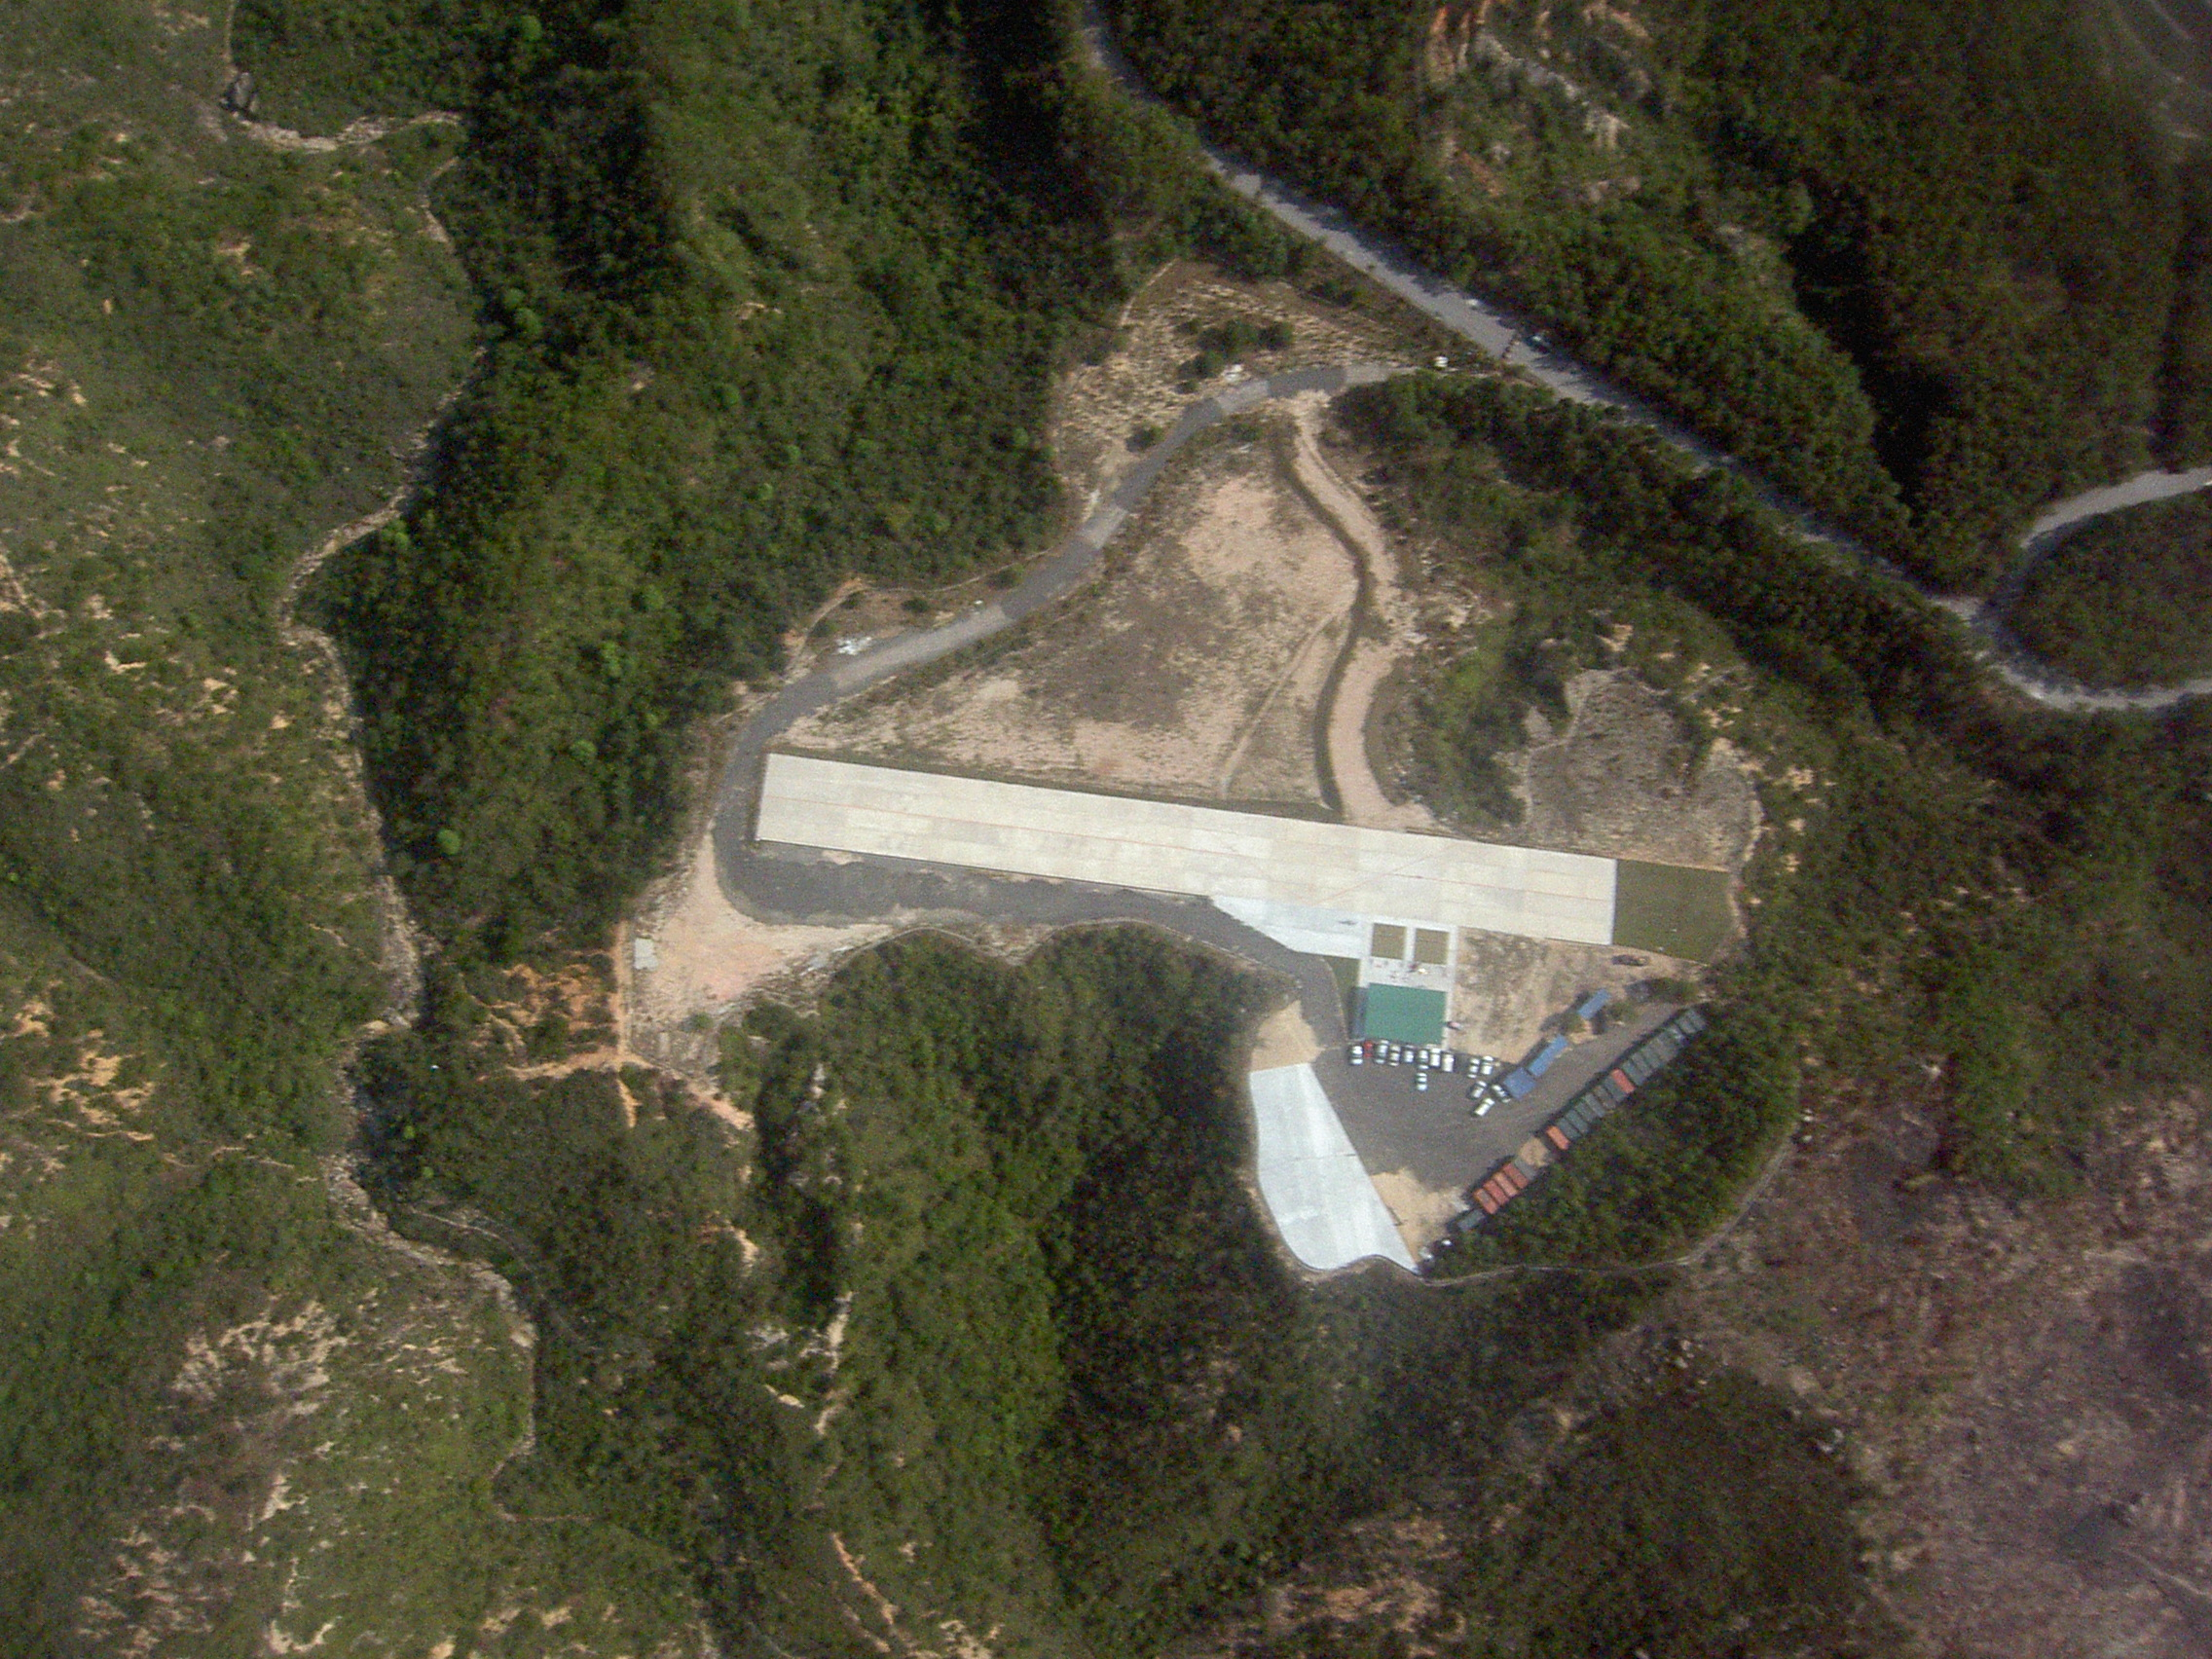
\includegraphics[height=1.9in]{asset/airfield.jpg}
        \caption{HKMEC airfield}
        \label{HKMEC}
    \end{minipage}
    \begin{minipage}{0.56\linewidth}
        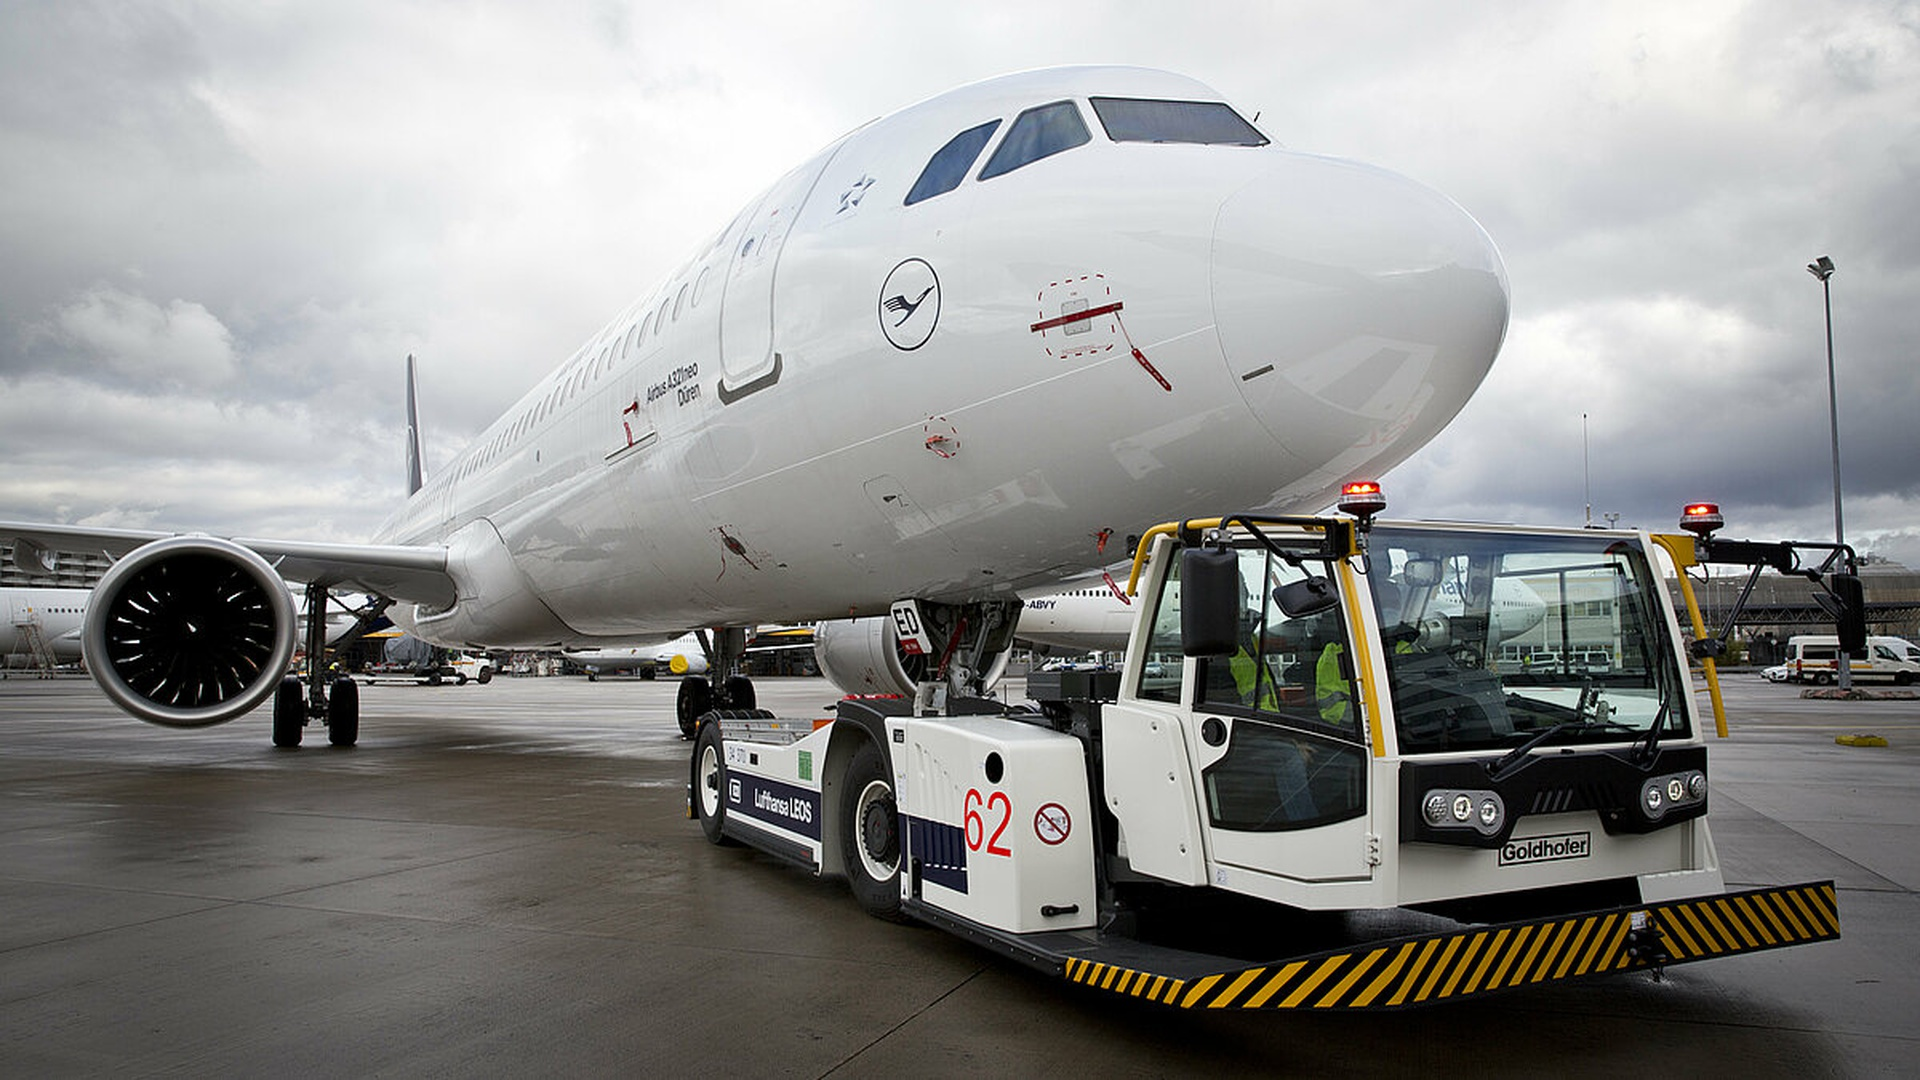
\includegraphics[height=1.9in]{asset/airplane.jpg}
        \caption{Tractor for real airplanes}
        \label{real_tractor}
    \end{minipage}
\end{figure}



}